%&program=xelatex
%&encoding=UTF-8 Unicode
% SVN keywords
% $Author$
% $Date$
% $Revision$
% $URL$
\documentclass[a4paper,twoside,12pt]{article}      % Comments after  % are ignored
%\usepackage{hyperref}                 % For creating hyperlinks in cross references
%
\usepackage{ifxetex}% for XELATEX, or PDFlatex
\usepackage{ifplatform} 
%
\ifxetex
	\usepackage{polyglossia} \setmainlanguage{portuges}
	\usepackage{fontspec}
	\ifwindows
		\setmainfont[Ligatures=TeX]{Garamond}
		\setsansfont[Ligatures=TeX]{Gill Sans MT}
		\setmonofont{Consolas}
%		\setmonofont[Scale=MatchLowercase]{Courier}
	\fi
	\iflinux
		\setmainfont[Ligatures=TeX]{Linux Libertine O}
		\setsansfont[Ligatures=TeX,Scale=MatchLowercase]{Linux Biolinum}
		\setmonofont[Scale=MatchLowercase]{Courier}
	\fi
	\ifmacosx
	% add settings
	% Use xelatex -no-shell ...
	\fi
	\usepackage{xcolor,graphicx} 
\else
	\usepackage[portuguese]{babel}
	%\usepackage[latin1]{inputenc}
	\usepackage[utf8]{inputenc}
	\usepackage[T1]{fontenc}
	\usepackage{graphics}                 % Packages to allow inclusion of graphics
	\usepackage{color}                    % For creating coloured text and background
\fi


\usepackage{amsmath,amssymb,amsfonts} % Typical maths resource packages
\usepackage{multicol}

\oddsidemargin 0cm
\evensidemargin 0cm

\pagestyle{myheadings}         % Option to put page headers
                               % Needed \documentclass[a4paper,twoside]{article}
\markboth{{\small \sf  Laboratório de Física Experimental Básica}}
{{\small\it MEFT - 2015/2016} }

\textwidth 15.5cm
\topmargin -1cm
\parindent 0.5cm
\textheight 24cm
\parskip 1mm

\usepackage{enumitem}
\setlist{nolistsep}

% Math macros
\newcommand{\ud}{\,\mathrm{d}} 
\newcommand{\HRule}{\rule{\linewidth}{0.5mm}}

\author{Prof. Bernardo B. Carvalho} 

%%%%, Bernardo Brotas Carvalho\\bernardo@ipfn.ist.utl.pt} 
\date{ Setembro 2012} 

\begin{document} 

%\begin{multicols}{1}
	
\includegraphics[width=0.2\textwidth]{../logo-ist}%\\[1cm]  %%  Logo_IST_color

		\HRule \\[0.5cm]
	{ \large \bfseries   \textsc{Estimativa da Carga Elétrica de 
		Gotículas de Óleo eletrizadas em Suspensão num Fluido (Experiência de Millikan)} }\\[0.4cm] % \bfseries 
	%{ \large  \sf 
%Ação de um campo elétrico sobre gotículas de óleo eletrizadas num fluido não 
%condutor. }\\
%	{ \large \bfseries Protocolo Experimental}\\
	\HRule \\%[0.5cm]

%	\HRule \\[0.5cm]
%	{ \huge \sf  \textsc{  Experiência de Millikan} }\\[0.4cm] % \bfseries 
%	{ \large \bfseries Determinação Experimental da Carga $q$ do Eletrão }\\
%	{ \large \bfseries Procedimento Experimental}\\
%	\HRule \\%[0.5cm]

%\twocolumn
%\end{multicols}

%\begin{multicols}{2}

\section{\sf OBJECTIVO DO TRABALHO}
Pretende-se com este trabalho determinar a carga elétrica de pequenas gotas de óleo, tendo como objectivo final mostrar que a carga elétrica não aparece com uma quantidade qualquer mas sempre como um múltiplo de uma unidade fundamental, que é a carga do eletrão. Deste modo, um corpo eletrizado apresenta um excesso de carga de sinal positivo ou negativo, mas sempre de valor múltiplo da carga elementar $q_{ele}= 1.602176565(35)\cdot 10^{-19}\,$ C.
Traduz-se este facto dizendo-se que a carga elétrica se \emph{quantifica}.

Dentro das várias experiências elaboradas para mostrar este facto, uma montagem clássica é a do físico americano Robert A. Millikan\footnote{Millikan recebeu o prémio Nobel da Física em 1923 pelos seus trabalhos sobre a determinação da carga do eletrão e efeito fotoelétrico.} (1869-1953), também chamada experiência da gota de óleo.

\section{\sf INTRODUÇÃO TEÓRICA}
%\section{\sf }
%\subsection{\sf }
\subsection{\sf Corpo esférico em queda livre num fluido}
Um corpo de dimensões muito pequenas,\footnote{Com Número de Reynolds $Re= \frac{\rho v L}{\eta}$ inferior a $\simeq 100$}  ao mover-se com uma velocidade relativamente baixa através de um fluido (líquido ou gás), fica sujeito a uma força de atrito aproximadamente proporcional à sua velocidade, modelada pela expressão:

\begin{equation}
	\label{eq:f_atrito}
	\vec{F}_{at} = - k \, \eta \vec{v}
\end{equation}
em que $\eta$ é o coeficiente de viscosidade do fluido, $\vec{v}$ é a velocidade do corpo e $k$ é um coeficiente que depende da forma do corpo, que no caso deste ser uma esfera de raio $R$ toma o valor (lei de Stokes): 
\begin{equation}
	\label{eq:coef_atrito}
	k = 6 \pi R
\end{equation}


O coeficiente $k$ virá assim expresso em \emph{metro} no Sistema Internacional (SI) e o coeficiente de viscosidade em Pa$\cdot$s (ou N$\cdot$s/m$^2$).
Normalmente a unidade de viscosidade que aparece na literatura é a unidade do sistema C.G.S. (g/cm$\cdot$s) que é designada por Poise (abreviatura P), verificando-se então a equivalência:

\begin{equation*}
	1 \, \mathrm{P} = 0.1\, \mathrm{Pa}\cdot\mathrm{s}
\end{equation*}

Quando um corpo de massa $m$ cai em queda livre sob a ação do seu peso ($\vec{P}=m\vec{g}$) através de um fluido, o seu movimento de queda será travado pela força de atrito, e a equação do movimento escreve-se:

\begin{equation}
	\label{eq:mov}
	m\,a \equiv m\, \frac{\ud\, v}{\ud\, t} =  m\,g - k  \, \eta \, v
\end{equation}

Sendo o peso do corpo constante, a aceleração $a$ produz um aumento  em $v(t)$ e por consequência, um aumento na força de atrito $F_{at}$. Para uma determinada velocidade limite $v_L$, o segundo membro de (\ref{eq:mov}) anula-se e o corpo passará a deslocar-se com movimento uniforme. A velocidade limite $v_L$ será então obtida fazendo na equação (\ref{eq:mov}) $a= 0$:

\begin{equation}
	\label{eq:vlimit}
	v_L = \frac{m\,g}{k  \, \eta}
\end{equation}
o que poderá ser facilmente constatado pela resolução da equação (\ref{eq:mov}), pois a sua solução é da forma:

\begin{equation}
	\label{eq:vlimita}
	v(t) = \frac{m\,g}{k  \, \eta} (1 - e^{- (k\,\eta / m) t})
\end{equation}
à qual corresponde o gráfico  da Fig~\ref{fig:vLim}. Quando $t \to \infty$ temos $v(t) \to v_L = \frac{m\,g}{k  \, \eta} $.


%\end{multicols}

\begin{figure}[tb]
  \centering 
	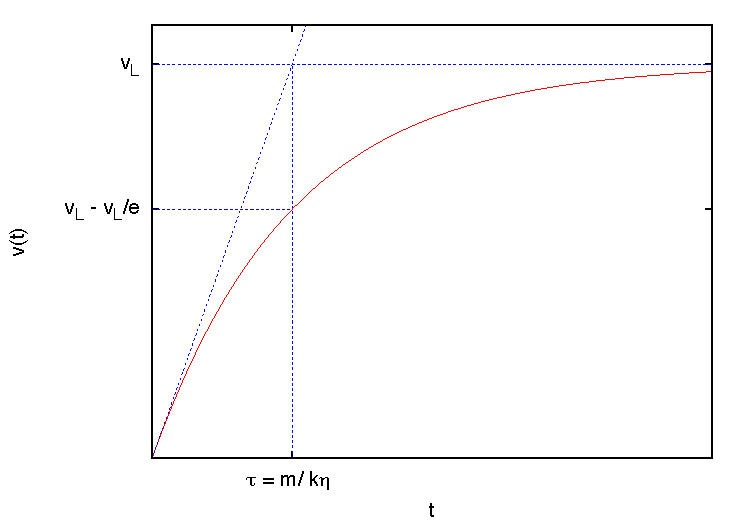
\includegraphics[width=0.6\textwidth]{./plote}
	\caption{ Evolução da velocidade de um corpo em queda livre sujeito a uma força de atrito. \label{fig:vLim}} 
\end{figure}

%\begin{multicols}{2}

Se pretendermos ser mais rigorosos devemos substituir  em (\ref{eq:vlimit}) o peso do corpo pelo seu “peso aparente” no fluido. De fato, quando um corpo cai em queda livre através de um fluido experimenta, além da ação da força de atrito, outra força de baixo para cima cujo módulo é igual ao peso do fluido deslocado pelo corpo, de acordo com o ''Princípio de Arquimedes''. Então  as equações (\ref{eq:mov}) e (\ref{eq:vlimit}) deverão ser modificadas para:

\begin{equation}
	\label{eq:mov2}
	m\,a = m\,g - m_f\,g  - k  \, \eta \, v
\end{equation}


\begin{equation}
	\label{eq:vlimit2}
	v_L = \frac{(m - m_f)\,g}{k  \, \eta}
\end{equation}
onde $m_f$ é a massa do fluido deslocado.

No caso de um corpo esférico de raio $R$, introduzindo a equação (\ref{eq:coef_atrito}) em (\ref{eq:vlimit2}) e atendendo a que:
\begin{equation*}
	m = \frac{4}{3} \pi R^3 \rho \quad \textrm{  e } \quad  m_f = \frac{4}{3} \pi R^3 \rho_f
\end{equation*}
obtemos
\begin{equation}
	\label{eq:vlimit3}
	v_L = \frac{2\,R^2\, (\rho - \rho_f)\,g}{9  \, \eta}
\end{equation}
em que $\rho$  e $\rho_f$ são as massas específicas do corpo e do fluido.

%

%\end{multicols}

\begin{figure}
	[tb]  \centering 
	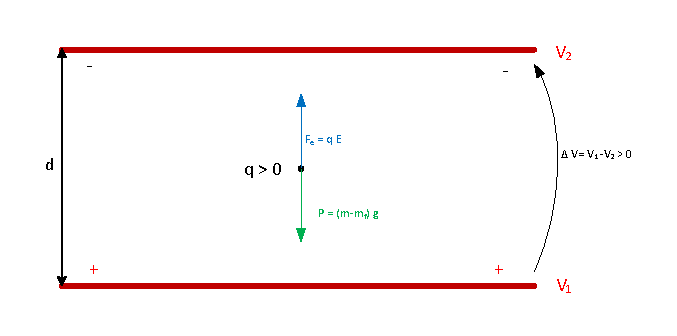
\includegraphics[width=0.7\textwidth]{./F_equil}
	\caption{Equilíbrio de forças elétrica e gravítica numa gota sujeita a campos gravítico e elétrico. \label{fig:f_equil}} 
\end{figure}

%\begin{multicols}{2}

\subsection{\sf Equilíbrio dum corpo carregado, imerso num fluido, através de um campo elétrico vertical.}

Considere o esquema representado na figura \ref{fig:f_equil}, em que entre duas placas condutoras paralelas se encontra um fluido não condutor. Aplica-se uma diferença de potencial \mbox{$U = V_1 -V_2 > 0$} com a polaridade indicada na figura. Esta diferença de potencial criará um campo elétrico ascendente. Se entre as placas se encontrar uma partícula de massa $m$ e carga positiva\footnote{No caso da partícula estar carregada negativamente obteríamos o mesmo resultado invertendo o sentido do campo elétrico.} $q$  esta ficará sujeita a uma força elétrica que contrariará a sua queda.
Na hipótese do campo elétrico ser uniforme\footnote{Nomeadamente, se a distância entre as placas muito menor que as suas dimensões laterais.} o módulo de $\vec{E}$ e o módulo da força elétrica $\vec{F}_e$ que atua na partícula serão dados por:


\begin{equation*}
	E = \frac{U}{d}, \qquad  F_e = |q| \frac{U}{d}
\end{equation*}
sendo $d$ a distância entre as placas. 

% O módulo a será então  dado por: 
% \begin{equation*}
% 	F = |q| \frac{U}{d}
% \end{equation*}

%Se a força elétrica for ascendente 
Assim, a queda da partícula será agora contrariada pela força elétrica e pela força de atrito.
A equação (\ref{eq:mov2}) passa a escrever-se:

\begin{equation}
	\label{eq:mov3}
	m\,a = (m - m_f)\,g  - q \frac{U}{d} - k  \, \eta_{ar} \, v
\end{equation}

Variando a diferença de potencial (ddp), $U$, pode-se estabelecer o equilíbrio entre o peso da partícula e a força elétrica, conseguindo-se a sua paragem entre as placas. Nesse caso tem-se $F_{at}$, $a$ e  $v$  $=0$:

\begin{equation}
	\label{eq:equil}
	0 = (m - m_f)\,g  - q \frac{U}{d} 
\end{equation}

Nesta equação a expressão $(m - m_f)\,g$ pode ser substituída usando a equação (\ref{eq:vlimit2}), obtendo-se:

\begin{equation*}
	v_L\, k\, \eta_{ar} = q \frac{U}{d}
\end{equation*}

E entrando também com a equação (\ref{eq:coef_atrito}) no caso de a partícula ser esférica, obtemos por fim:

\begin{equation}
	\label{eq:carga}
	q = \frac{6 \pi \, R \, \eta_{ar} \, d\, v_L}{U}  
\end{equation}
onde

\begin{itemize}
\item $v_L$, a velocidade limite de queda da partícula através do fluido, na ausência do campo elétrico
\item $\eta_{ar} = 18.52 \cdot 10^{-5}$ P $=  18.52 \cdot 10^{-6} \;$ Pa$\cdot$s (Viscosidade do ar a 23 $^{\circ}$C)
\item $\rho = 973 \,$ kg/m$^{3}$ (Massa específica do óleo de silicone)
\item $\rho_f = 1 \,$ kg/m$^{3}$ (Massa específica do ar)
\item $g=9.80\,$ m/s$^{2}$ (Aceleração gravítica em Lisboa)
\item $d$ (Distância entre placas a medir no Laboratório)
\end{itemize}

\subsection{\sf Correções.}
\subsubsection{\sf Temperatura Ambiente.}

O valor  da viscosidade do ar, no caso da temperatura ambiente se afastar muito de $23\,^{\circ}\mathrm{C}$, terá de ser corrigido.\footnote{Utilize por exemplo a calculadora \emph{online}: http://www.lmnoeng.com/Flow/GasViscosity.htm}

\subsubsection{\sf Dimensão das gotas.}

A Lei de Stokes não é exata quando as dimensões dos corpos esféricos forem comparáveis à distância média entre as moléculas do ar. Nestas condições, Millikan verificou que a viscosidade $\eta_{ar}$ deveria ser substituída por:

\begin{equation}
	\label{eq:correcao}
	\eta_{ar}' = \frac{\eta_{ar}}{1 + b/(p\,R)}  
\end{equation}
em que a constante $b=7.88\cdot 10^{-3}$ Pa$\cdot$m, 
$p$ é pressão atmosférica expressa em pascal e $R$ é o raio da gota em metros.
%$0.000617$, $p$ é pressão expressa em $cm$ de %mercúrio\footnote{$1\,atm  = 1.013 \times 10^5 \,Pa = %1013 \, mbar %= 76\, cm_{Hg}$}  e $R$ é o raio da gota em %$cm$.

O valor corrigido $q'$ será  determinado a partir do valor experimental $q$ por

\begin{equation}
	\label{eq:correcao1}
	q' = q\, \left(\frac{\eta_{ar}'}{\eta_{ar}}\right)^{3/2}  =q\, \left(\frac{1}{1 + b/(p\,R)}\right)^{3/2}  
\end{equation}

\begin{figure}
	[htb]  \centering 
	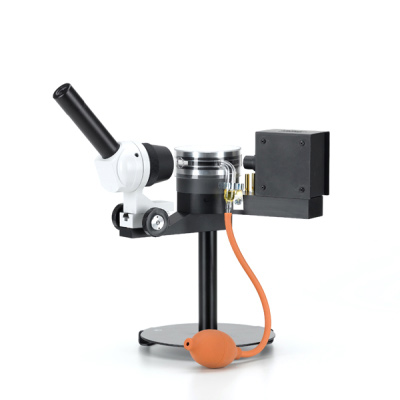
\includegraphics[width=0.5\textwidth]{./U131001_01_Aparelho-de-Millikan}
	\caption{Equipamento para determinação da carga de gotas. \label{fig:Equi}} 
\end{figure}

\begin{figure}
	[htb]  \centering 
	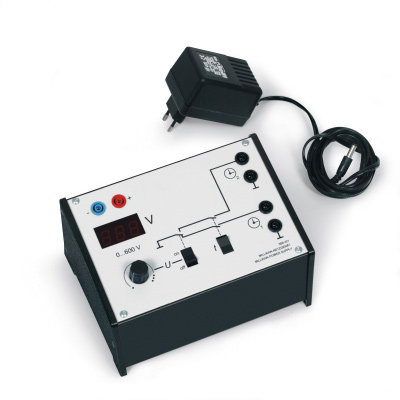
\includegraphics[width=0.5\textwidth]{./U13105-230_01_Aparelho-operacional-de-Millikan}
	\caption{Gerador de alta tensão DC regulável. \label{fig:fonteDC_HT}} 
\end{figure}


\newpage
\section{\sf Procedimento Experimental}


\subsection{\sf Material utilizado}

\begin{enumerate}
	\item Célula de Millikan com gerador de alta tensão DC regulável
	\item  Atomizador e óleo de silicone
	\item Cronómetro
	\item Nível de bolha de ar% Parafuso para calibração do retículo do microscópio
\end{enumerate}
\section{\sf Procedimento experimental}

\begin{enumerate}
\item   Depois de verificar que a célula está horizontal, meça a distância entre placas, $d$. Tente focar o microscópio na zona onde as gotas irão ``flutuar''. (Atenção que o microscópio amplia a imagem e a escala por 2$\times$).
\item Coloque o potenciómetro que 
controla a alimentação das placas do condensador no valor mínimo de tensão elétrica. 
\item    Verifique se o interruptor de inversão da alimentação do condensador está na posição ``Neutra''.
Rode o potenciómetro para uma posição que permita, quando ligar o interruptor de inversão, estabelecer um campo elétrico entre as placas do condensador. 
\item     Utilizando o pulverizador junto do orifício da célula produza uma pequena ``nuvem'' %“nuvem”
de gotículas de óleo. Observe através do microscópio o movimento das gotículas em 
frente do retículo.
\item     Ligando o interruptor e variando a intensidade  e o  sentido do campo elétrico, Verifique se existem gotículas eletrizadas. Escolha uma das gotas e tente pará-la.
 \item Obrigue a gota a colocar-se numa determinada divisão do retículo, imobilizando-a. 
Leia o valor da diferença de potencial que permitiu essa imobilização. Anule o 
campo elétrico  e verá a gota movimentar-se (com velocidade limite). Com a ajuda de um colega e um 
cronómetro, meça o tempo necessário para que a gota percorra  $N>4$ divisões
do retículo. Repondo o campo elétrico, conduza a gota para a posição inicial para  medir o tempo pelo menos duas vezes. 
\item Troque de posição com o colega para repetir este processo para várias gotas, tentando escolher as gotas de menor carga.
\item   Calcule a velocidade limite média de cada gota e a respetiva incerteza. Estime o raio e 
a carga de cada gota e correspondentes incertezas. Calcule a carga corrigida pela viscosidade.
\item   Compare os valores da carga média das gotas de menor carga  com o valor tabelado da carga do eletrão. 
\end{enumerate}



%\end{multicols}

\end{document} 